\documentclass[12pt,letterpaper]{article}

\usepackage[utf8]{inputenc}
\usepackage[spanish]{babel}
\usepackage{graphicx}
\usepackage{geometry}
\usepackage{amsmath}
\usepackage{float}
\usepackage{caption}
\usepackage{subcaption}
\usepackage{setspace}
\usepackage{csquotes}
\usepackage{booktabs}
\usepackage{titling}    % <-- debe estar presente
\usepackage{siunitx}
\usepackage[backend=biber,style=ieee]{biblatex}
\addbibresource{references.bib}

\geometry{left=2.5cm, right=2.5cm, top=2.5cm, bottom=2.5cm}

\title{Análisis de Tejidos mediante Tomografía Fotoacústica e IA\\
Integración de un Sistema Propio de Adquisición de Datos}
\author{Eduardo Santos Mena \\ Asesores: Dr. Samuel Pérez Huerta, Dr. Augusto David Ariza Flores}
\date{Reporte de Avance - Tercer Semestre 2025}

\begin{document}

\maketitle

\begin{abstract}
\noindent
El presente reporte documenta la evolución técnica del sistema de tomografía fotoacústica (PAT), marcando la transición desde la validación óptica preliminar hacia la consolidación de una arquitectura de instrumentación electrónica propietaria. Con el objetivo de superar las limitaciones de control y sincronización inherentes a la instrumentación comercial genérica, se desarrolló la versión 2.0 de la fuente de excitación óptica. Esta iteración integra una lógica de control embebida (RP2040) para la orquestación precisa de disparos y un sistema de retroalimentación óptica mediante fotodiodo y amplificador de transimpedancia para el monitoreo de potencia \textit{in-situ}. Paralelamente, se diseñó e implementó una cadena de adquisición de datos autónoma, constituida por una etapa de acondicionamiento analógico selectivo (ancho de banda de 194\,kHz a 3.38\,MHz) optimizada para transductores de 2.5\,MHz, y un núcleo de procesamiento digital basado en FPGA. La validación rigurosa del sistema, mediante protocolos de integridad de señal, respuesta dinámica y linealidad estática ($R^2 \approx 1.0$), demuestra la fiabilidad del diseño lógico y la ausencia de pérdida de datos. Estos avances establecen una plataforma experimental robusta, modular y de bajo costo, sentando las bases tecnológicas para la integración del conversor analógico-digital y la caracterización futura de fantomas biológicos.

En esencia, este desarrollo valida la factibilidad de sustituir plataformas comerciales cerradas y de alto costo por una arquitectura de instrumentación abierta. Este enfoque reduce drásticamente la barrera económica de entrada y otorga acceso total a los parámetros de diseño, permitiendo una personalización instrumental ("fine-tuning") inaccesible en equipos genéricos.

\end{abstract}

\newpage
\section{Introducción}

La tomografía fotoacústica (PAT) combina la especificidad molecular de la excitación óptica con la resolución de la detección ultrasónica, ofreciendo un potencial significativo para el diagnóstico temprano de patologías como la artritis reumatoide mediante la visualización de la neovascularización sinovial~\cite{lin_emerging_2022}. 

Durante el semestre anterior, la validación de una fuente basada en láseres LED de 445\,nm confirmó la viabilidad técnico-económica de la generación de pulsos ópticos de bajo costo~\cite{wu_advanced_2021}~\cite{li_photoacoustic_2020}. No obstante, se identificó una limitación crítica en la arquitectura experimental: la dependencia de instrumentación de laboratorio de propósito general (osciloscopios comerciales). Dichos equipos actúan como "cajas negras" en el procesamiento de señal, restringiendo la sincronización determinista y el control de tiempos (\textit{timing control}) necesarios para implementar algoritmos de reconstrucción tomográfica de alta fidelidad.

En respuesta a estas limitaciones, la investigación en este tercer periodo pivotó hacia la ingeniería de instrumentación, enfocándose en el desarrollo de un \textit{sistema de adquisición de datos (DAQ) propietario} y la evolución de la electrónica de control. Este cambio estratégico hacia una arquitectura de hardware dedicado permite:

\begin{enumerate}
    \item \textbf{Autonomía y Sincronización:} La eliminación de generadores de funciones externos mediante la integración de lógica de disparo embebida (RP2040) garantiza una latencia mínima y determinista entre la excitación óptica y el inicio de la adquisición acústica.
    \item \textbf{Fidelidad de Señal (SNR):} El diseño de una etapa de acondicionamiento analógico (\textit{Analog Front-End}) con ancho de banda selectivo para el transductor ultrasónico supera las capacidades de los filtros digitales genéricos, maximizando la relación señal-ruido antes de la digitalización.
    \item \textbf{Control Digital Flexible:} La gestión directa de la temporización de muestreo mediante FPGA habilita la implementación futura de técnicas de promediado de señales en hardware (\textit{hardware-based averaging}), esenciales para recuperar señales fotoacústicas débiles en entornos ruidosos.
\end{enumerate}

El presente reporte detalla el diseño e implementación del Driver V2.0 con retroalimentación óptica, el cálculo y fabricación de la etapa de filtrado analógico sintonizada, y el protocolo de validación rigurosa del núcleo digital del sistema.

\section{Objetivos del Periodo}

El objetivo general de esta etapa fue establecer y validar una plataforma de hardware propietaria capaz de gestionar la cadena completa de adquisición fotoacústica, desde el disparo óptico hasta la digitalización de la señal.

Los objetivos específicos alcanzados fueron:

\begin{enumerate}
    \item \textbf{Evolución de la Fuente de Excitación (Driver V2.0):} Integrar en un PCB unificado la etapa de potencia, la lógica de control basada en microcontrolador y un sistema de monitoreo de potencia óptica en tiempo real mediante amplificador de transimpedancia (TIA).
    \item \textbf{Diseño de Acondicionamiento Analógico:} Calcular e implementar una cadena de filtrado híbrida (pasiva/activa) sintonizada específicamente para la respuesta en frecuencia de transductores de 2.5\,MHz, optimizando el rechazo a ruido fuera de banda.
    \item \textbf{Validación del Núcleo Digital (FPGA):} Certificar la integridad de datos, la linealidad de la conversión y la respuesta dinámica del protocolo de comunicación FPGA-PC mediante pruebas unitarias, asegurando la fiabilidad del sistema antes de la experimentación biológica.
\end{enumerate}
\section{Metodología y Desarrollo}

\subsection{Optimización de Fuente de Excitación (Driver V2.0)}
Se rediseñó el driver de corriente desarrollado en la etapa anterior para operar como un módulo autónomo y robusto. Las mejoras críticas implementadas en esta iteración incluyen:

\begin{itemize}
    \item \textbf{Control Embebido:} Incorporación de un microcontrolador RP2040 directamente en el PCB. Esto permite la generación de \textit{triggers} programables por software, eliminando el \textit{jitter} y la latencia asociados al cableado de generadores de funciones externos.
    \item \textbf{Gestión Térmica:} Adición de resistencias de potencia dedicadas para estabilizar la descarga inductiva del circuito, mejorando la disipación de calor y permitiendo operaciones prolongadas sin deriva térmica significativa.
    \item \textbf{Estimación de Potencia:} Integración de un fotodiodo con amplificador de transimpedancia (TIA) embebido en la placa. Este subsistema recibe una derivación óptica mediante fibra, permitiendo medir la energía real emitida pulso a pulso para la normalización de señales posterior.
\end{itemize}

% [PLACEHOLDER FIGURA 1 y 2]
% Aquí irían las fotos del PCB o el diagrama de bloques del Driver V2
% \begin{figure}[H]
%    \centering
%    \includegraphics[width=0.8\textwidth]{nombre_imagen_driver.png}
%    \caption{Arquitectura del Driver V2.0 mostrando la integración del control digital y la retroalimentación óptica.}
%    \label{fig:driver_v2}
% \end{figure}

\subsection{Diseño de Etapa de Filtrado}
Para adaptar la cadena de adquisición a un transductor ultrasónico de 2.5\,MHz, fue necesario rediseñar la etapa de entrada analógica. El objetivo de diseño fue implementar un filtro pasa-banda que elimine el ruido mecánico de baja frecuencia ($<200\,kHz$) y evite el \textit{aliasing} digital atenuando frecuencias superiores a 3.5\,MHz.

\subsubsection{Filtro Pasa Altas (Pasivo RC)}
Se diseñó un filtro de primer orden a la entrada para eliminar componentes de DC y vibraciones mecánicas. Utilizando un capacitor comercial $C_4 = 1\,\text{nF}$, se calculó la resistencia $R_{13}$ necesaria para la frecuencia de corte deseada:

\begin{equation}
    f_{c_{Pa}} = \frac{1}{2\pi R_{13} C_4} \approx 194\,\text{kHz}
\end{equation}

Para la implementación física, se seleccionó el valor comercial más cercano de $R_{13} = 820\,\Omega$.

\subsubsection{Filtro Pasa Bajas (Activo Sallen-Key)}
Para limitar el ancho de banda superior, se implementó un filtro activo de segundo orden en configuración Sallen-Key. Asumiendo una topología de ganancia unitaria y capacitores estándar para RF de $C_2=C_3=100\,\text{pF}$, se determinó el valor de las resistencias $R_{11,12}$:

\begin{equation}
    f_{c_{Pb}} = \frac{1}{2\pi \sqrt{R_{11}R_{12}C_2 C_3}} \approx 3.38\,\text{MHz}
\end{equation}

Se seleccionaron valores comerciales de $R_{11} = R_{12} = 470\,\Omega$.

% [PLACEHOLDER FIGURA 3]
% Aquí se hará referencia a la simulación o esquemático del filtro
% \begin{figure}[H]
%    \centering
%    \includegraphics[width=0.8\textwidth]{analog_filtering_schematic.png}
%    \caption{Esquemático de la etapa de filtrado analógico sintonizada para 2.5 MHz.}
%    \label{fig:filter_schematic}
% \end{figure}
\subsection{Arquitectura del Núcleo Digital (FPGA)}

Para dotar al sistema de capacidades de adquisición determinista, se diseñó una arquitectura lógica propietaria en Verilog. A diferencia de los sistemas de adquisición continua, este diseño implementa una estrategia de \textbf{"Store-and-Forward"} (Almacenar y Reenviar) que optimiza el uso del ancho de banda disponible.

\subsubsection{Lógica de Adquisición (Store-and-Forward)}
El sistema explota el bajo ciclo de trabajo del láser de excitación para desacoplar la velocidad de muestreo de la velocidad de transmisión. Como se ilustra en el diagrama de flujo (Figura \ref{fig:logic_flow}), la Máquina de Estados Finitos (FSM) opera en tres fases cíclicas:

\begin{enumerate}
    \item \textbf{IDLE (Reposo):} El sistema monitoriza la entrada de \textit{trigger} externo (5 kHz), manteniendo los punteros de memoria reiniciados.
    \item \textbf{CAPTURE (Burst Mode):} Al detectar un flanco de subida, el FPGA activa el ADC a su velocidad nominal (27 Msps) y llena un bloque de memoria RAM interna (\textit{Block RAM}) con 2048 muestras. Esta ventana temporal ($\approx 75\,\mu s$) es suficiente para capturar la profundidad de penetración óptica máxima teórica.
    \item \textbf{SENDING (Transmisión):} Durante el tiempo muerto entre pulsos láser ($\approx 125\,\mu s$), la FSM detiene la adquisición y transmite los datos almacenados hacia la PC mediante una interfaz UART estándar a 115200 baudios.
\end{enumerate}

\begin{figure}[H]
    \centering
    \includegraphics[width=0.85\textwidth]{figuras/fgpa_daq_system.png}
    \caption{Arquitectura "Store-and-Forward". El diseño aprovecha los tiempos muertos del láser para transmitir datos de alta velocidad a través de una interfaz serial estándar.}
    \label{fig:logic_flow}
\end{figure}

\subsubsection{Protocolo de Validación Unitaria}
Antes de la integración con la etapa analógica, se definió un protocolo de pruebas unitarias para certificar la fiabilidad del núcleo digital. Se diseñaron tres experimentos de control mediante la generación de señales sintéticas internas (\textit{Virtual ADC}):

\begin{itemize}
    \item \textbf{Exp. A (Integridad):} Generación de un patrón de contador incremental de 8 bits para verificar la ausencia de pérdida de paquetes (\textit{packet loss}) en el enlace UART.
    \item \textbf{Exp. B (Linealidad):} Simulación de un barrido de voltaje DC (0-255 LSB) para evaluar la precisión de decodificación y la estabilidad del bus de datos.
    \item \textbf{Exp. C (Dinámica):} Inyección de una señal senoidal digital para verificar el cumplimiento de los tiempos de \textit{setup/hold} a 27 MHz y la correcta reconstrucción de señales AC.
\end{itemize}

\section{Resultados}

La validación del sistema se presenta en tres bloques: la implementación de la electrónica de potencia y control (Driver V2.0), la respuesta en frecuencia de la etapa analógica y la certificación del núcleo digital (FPGA).

\subsection{Implementación del Driver de Excitación V2.0}
Se completó el diseño del circuito de excitación integrando la lógica de control y la etapa de potencia. Como se muestra en el esquema de la etapa de retroalimentación (Figura \ref{fig:feedback_schematic}), el sistema incluye un amplificador de transimpedancia (TIA) acoplado directamente al microcontrolador. Esta configuración permite la lectura del fotodiodo monitor con una latencia despreciable, habilitando la corrección de fluctuaciones de potencia pulso a pulso, una funcionalidad ausente en la versión anterior.

\begin{figure}[H]
    \centering
    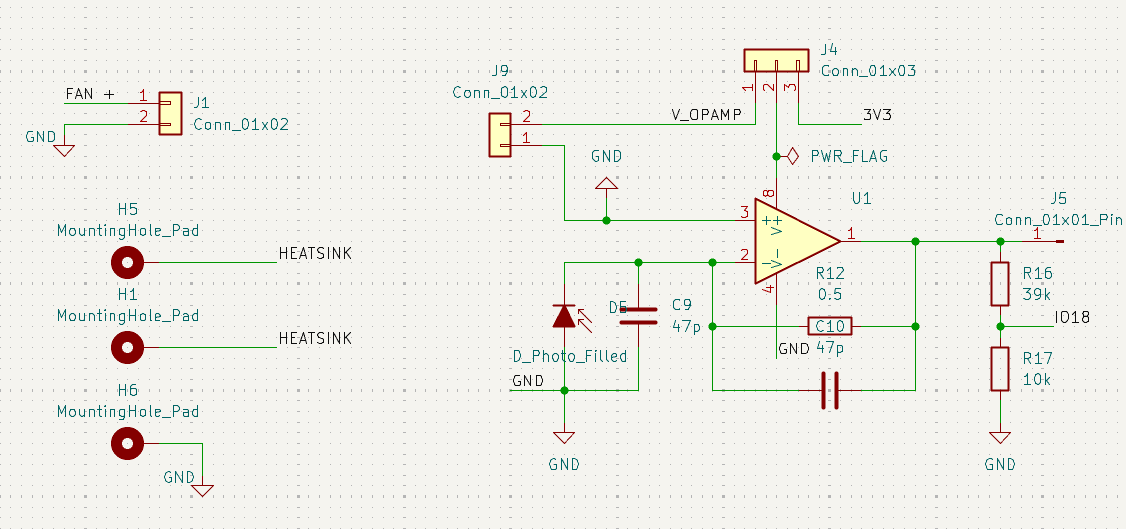
\includegraphics[width=0.9\textwidth]{figuras/retroalimentacion_current_drive.png}
    \caption{Esquemático de la etapa de retroalimentación óptica embebida en el Driver V2.0. El fotodiodo captura una fracción del pulso láser, y la señal acondicionada es digitalizada por el microcontrolador para estimación de energía en tiempo real.}
    \label{fig:feedback_schematic}
\end{figure}

\subsection{Diseño y Respuesta de la Etapa Analógica}

La cadena de acondicionamiento analógico se implementó en dos fases: pre-amplificación y filtrado selectivo. La Figura \ref{fig:analog_schematics} detalla la topología circuital diseñada. 

En la primera etapa (Figura \ref{fig:sch_amp}), se empleó un amplificador de instrumentación para elevar el nivel de la señal proveniente del transductor piezoeléctrico, garantizando una alta impedancia de entrada. Posteriormente, la señal pasa a la etapa de filtrado (Figura \ref{fig:sch_filter}), donde se configuró la red híbrida recalculada: un filtro pasa-altas pasivo ($R=820\,\Omega, C=1\,\text{nF}$) para el rechazo de DC y ruido mecánico, seguido de un filtro activo Sallen-Key ($R=470\,\Omega, C=100\,\text{pF}$) para limitar el ancho de banda.

\begin{figure}[H]
    \centering
    \begin{subfigure}[b]{0.48\textwidth}
        \centering
        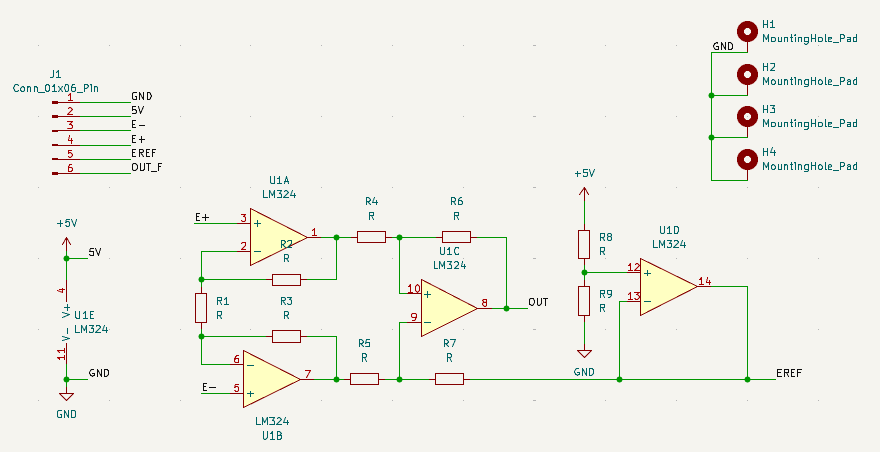
\includegraphics[width=\textwidth]{figuras/amplificador_instrumentacion.png}
        \caption{Amplificador de Instrumentación}
        \label{fig:sch_amp}
    \end{subfigure}
    \hfill
    \begin{subfigure}[b]{0.48\textwidth}
        \centering
        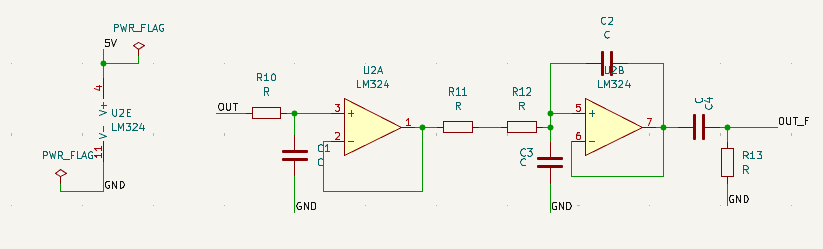
\includegraphics[width=\textwidth]{figuras/filtro.png}
        \caption{Filtros Pasa-Altas y Pasa-Bajas}
        \label{fig:sch_filter}
    \end{subfigure}
    \caption{Esquemáticos de la etapa de acondicionamiento analógico. (a) Etapa de ganancia inicial. (b) Configuración de filtrado sintonizada para la ventana de 194 kHz - 3.39 MHz.}
    \label{fig:analog_schematics}
\end{figure}

La validación espectral de este diseño (Figura \ref{fig:analog_sim}) confirma que la topología satisface los requerimientos para el transductor de 2.5 MHz. La simulación muestra que los polos ubicados en $\approx 194$\,kHz y $\approx 3.39$\,MHz crean una ventana espectral que maximiza la relación señal-ruido (SNR) antes de la digitalización, evitando el \textit{aliasing} sin atenuar la portadora ultrasónica principal.

\begin{figure}[H]
    \centering
    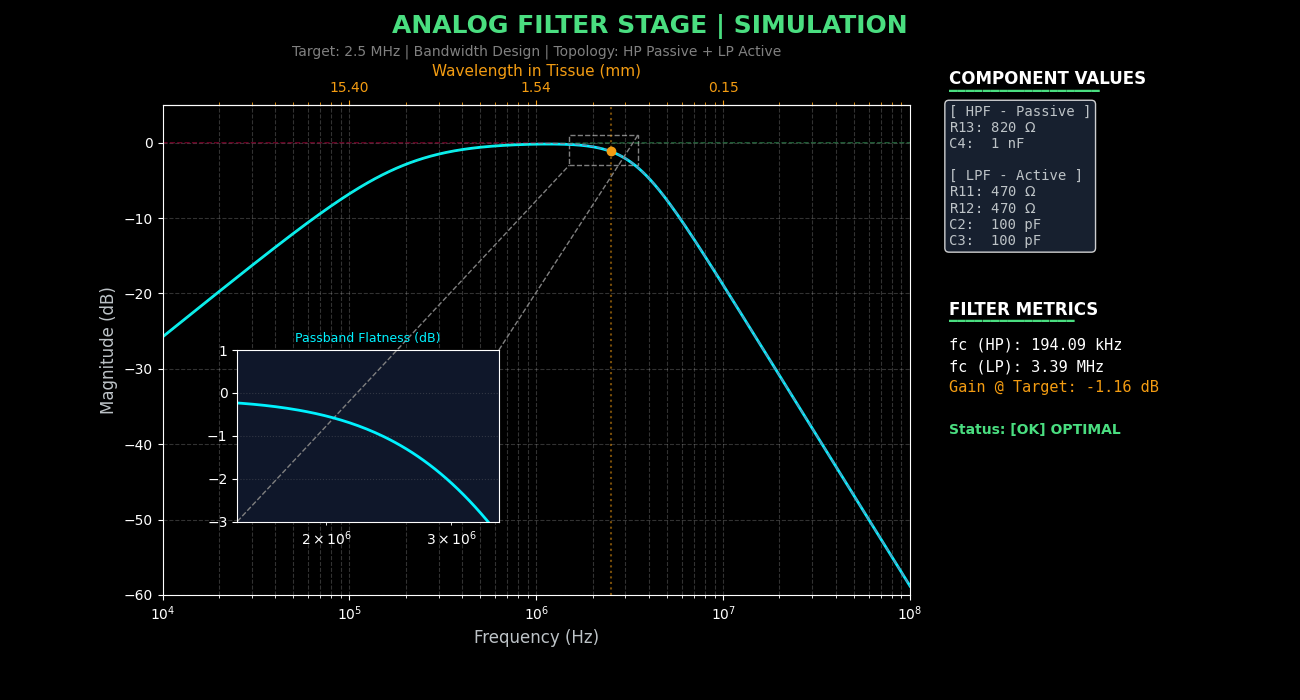
\includegraphics[width=0.95\textwidth]{figuras/analog_filtering.png}
    \caption{Respuesta en frecuencia simulada del circuito completo. Se observa la banda de paso plana centrada en 2.5 MHz, coincidiendo con los cálculos de diseño.}
    \label{fig:analog_sim}
\end{figure}



\subsection{Validación del Núcleo Digital (FPGA)}
A continuación se presentan los resultados de los tres experimentos unitarios diseñados para certificar el desempeño del sistema de adquisición propietario.

\subsubsection{Integridad de Transmisión (Exp. A)}
La ejecución del protocolo de integridad (Figura \ref{fig:sawtooth}) resultó en la reconstrucción de una señal de "diente de sierra" monótona. El análisis de la ventana de muestreo (correlacionada con 5.84 cm de profundidad teórica en tejido) confirma que:
1. No existen discontinuidades en la secuencia numérica (Pérdida de bytes = 0\%).
2. La sincronización entre el FPGA y el software de visualización es robusta, validando la gestión de los punteros de memoria RAM interna.

\begin{figure}[H]
    \centering
    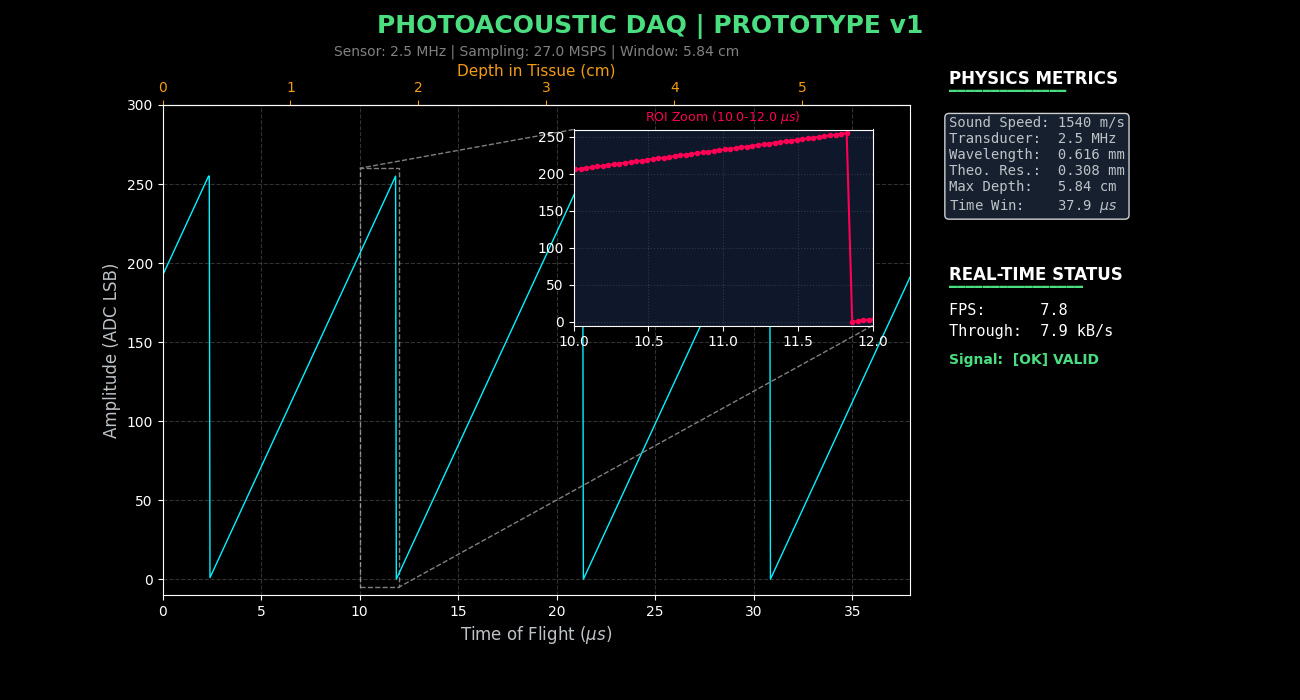
\includegraphics[width=1.0\textwidth]{figuras/FPGA_DAQ_SAW.png}
    \caption{Resultado de la prueba de integridad digital. La continuidad perfecta de la rampa en la ventana de adquisición confirma una transmisión UART libre de errores.}
    \label{fig:sawtooth}
\end{figure}

\subsubsection{Linealidad Estática (Exp. B)}
El análisis de regresión sobre el barrido digital (Figura \ref{fig:linearity}) arrojó un coeficiente de determinación $R^2 = 1.00000$. El gráfico de residuos muestra un error máximo de cuantización de 0.37 LSB, lo cual es inherente al proceso de digitalización y despreciable para la aplicación. Esto valida que el mapeo entre el voltaje de entrada (simulado) y el código digital es estrictamente lineal.

\begin{figure}[H]
    \centering
    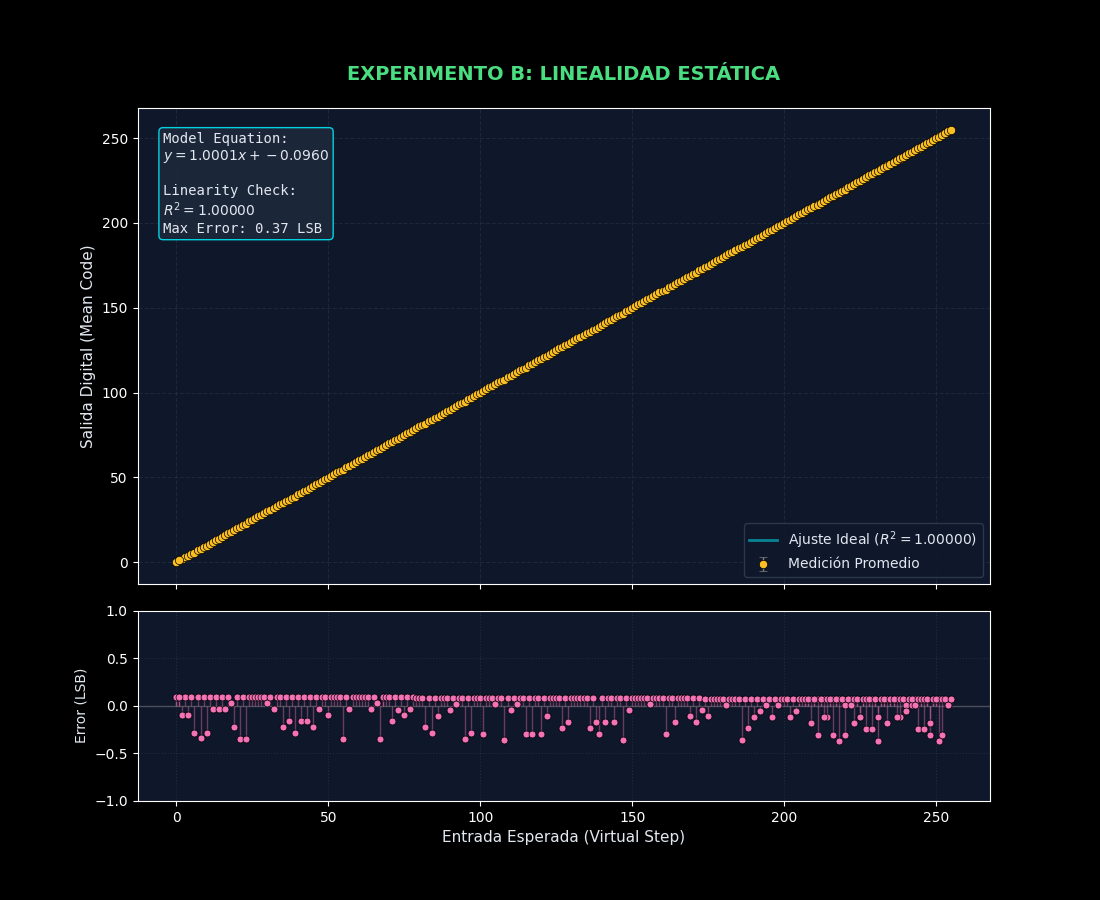
\includegraphics[width=0.85\textwidth]{figuras/error_lsb.png}
    \caption{Análisis de error de linealidad estática. La desviación mínima respecto al ajuste ideal valida la precisión matemática de la decodificación de datos en el FPGA.}
    \label{fig:linearity}
\end{figure}

\subsubsection{Respuesta Dinámica y Ancho de Banda (Exp. C)}
La reconstrucción de la señal senoidal sintética (Figura \ref{fig:dynamic}) demuestra la capacidad del sistema para procesar señales rápidas. El análisis en el dominio de la frecuencia (FFT inferior) muestra picos espectrales limpios en la fundamental (421.9 kHz) y sus armónicos, confirmando el correcto funcionamiento del reloj de muestreo a 27 MHz y el cumplimiento de los tiempos de \textit{setup/hold} en la lógica interna.

\begin{figure}[H]
    \centering
    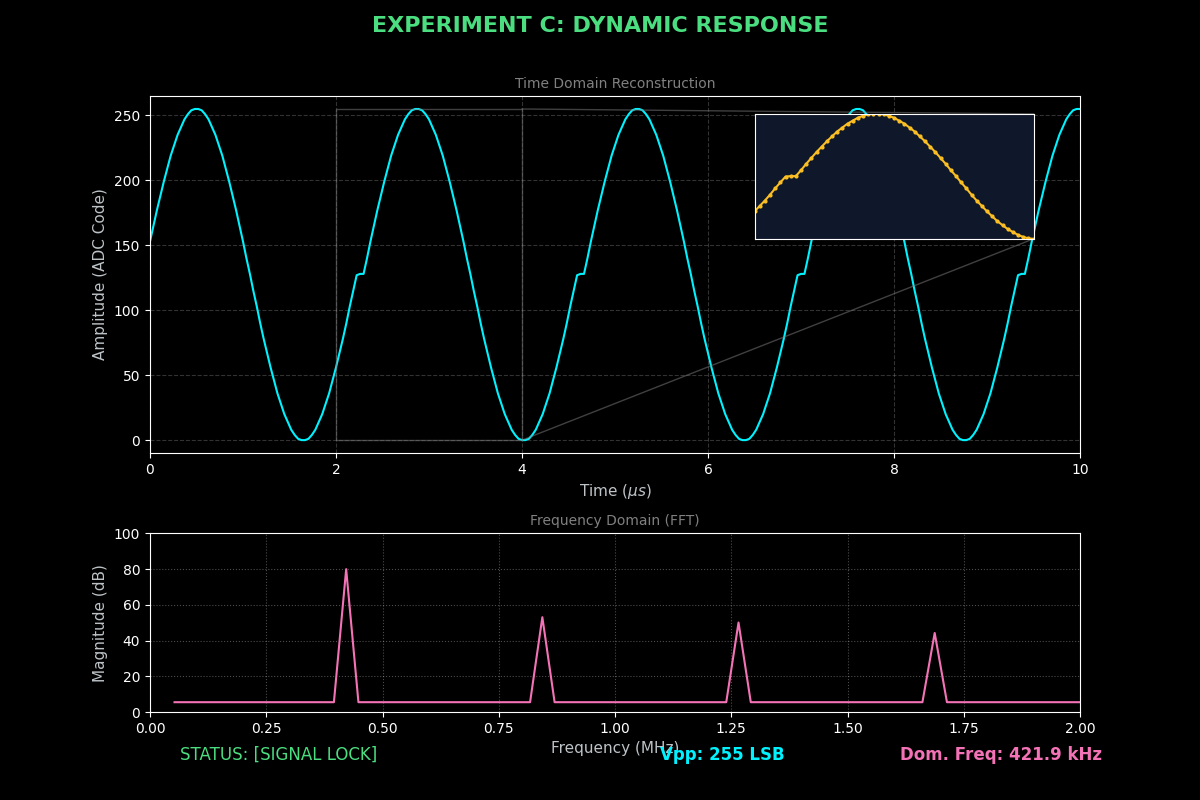
\includegraphics[width=1.0\textwidth]{figuras/experimento_c.png}
    \caption{Validación de respuesta dinámica. La reconstrucción exitosa de la forma de onda AC y su espectro confirman que el ancho de banda digital es suficiente para capturar pulsos fotoacústicos.}
    \label{fig:dynamic}
\end{figure}

\section{Discusión}

\subsection{Síntesis de Hallazgos}
La transición estratégica hacia el desarrollo de hardware propietario ha dotado al proyecto de una "caja blanca" (FPGA) frente a la "caja negra" (osciloscopio) utilizada en etapas anteriores. Los resultados de la validación unitaria confirman que el núcleo digital desarrollado es determinista y preciso. Específicamente, la prueba de integridad (Exp. A) y el análisis de linealidad ($R^2=1.0000$) demuestran que la arquitectura de adquisición "Store-and-Forward" gestiona correctamente el flujo de datos sin pérdida de información, validando el uso de la memoria interna del FPGA como \textit{buffer} intermedio.

\subsection{Interpretación e Impacto Técnico}
El diseño de la etapa de acondicionamiento analógico representa una mejora sustancial respecto a la conexión directa utilizada previamente. La implementación de una ventana espectral selectiva ($194\,\text{kHz} - 3.39\,\text{MHz}$) permite rechazar el ruido vibracional de baja frecuencia y el ruido térmico de alta frecuencia antes de la digitalización, lo cual es crítico dado que las señales fotoacústicas en tejidos profundos suelen tener amplitudes del orden de microvoltios.

Adicionalmente, la evolución del Driver V2.0 resuelve una incertidumbre mayor del semestre anterior: la estabilidad de la potencia óptica. La integración del fotodiodo con amplificador de transimpedancia (TIA) permite ahora correlacionar cada señal acústica adquirida con la energía real del pulso láser que la generó, habilitando técnicas de normalización que reducirán variaciones estocásticas en las imágenes futuras.

\subsection{Limitaciones Actuales}
La principal limitación del prototipo actual reside en el ancho de banda de transmisión hacia la PC. La interfaz UART a 115200 baudios impone un cuello de botella que impide la visualización en tiempo real a la velocidad máxima de muestreo del ADC (65 Msps). Actualmente, el sistema opera mediante captura por ráfagas y transmisión diferida. Si bien esto es suficiente para la validación estática y adquisiciones de baja tasa de repetición, la implementación futura de visualización en vivo requerirá el uso de interfaces de mayor velocidad (USB 2.0/3.0) o compresión de datos en hardware. Asimismo, la validación presentada se limita al dominio eléctrico; la respuesta acústica real dependerá del acoplamiento físico del transductor, que se abordará en la siguiente fase.

\section{Conclusiones}

Se ha completado con éxito la fase de ingeniería de instrumentación, estableciendo una plataforma de hardware propietaria y validada para la investigación en tomografía fotoacústica.

\begin{enumerate}
    \item \textbf{Autonomía Instrumental:} El desarrollo del Driver V2.0 y el DAQ basado en FPGA elimina la dependencia de equipos comerciales costosos, reduciendo el costo del prototipo y aumentando la flexibilidad de control experimental.
    \item \textbf{Robustez Digital:} Los protocolos de validación unitaria certifican que el sistema de adquisición es lineal, estable y libre de errores de transmisión, cumpliendo con los requisitos de integridad de datos para aplicaciones científicas.
    \item \textbf{Optimización Analógica:} El recálculo y simulación de los filtros analógicos aseguran una adaptación de impedancia y frecuencia óptima para los transductores de 2.5 MHz, maximizando la relación señal-ruido teórica.
\end{enumerate}

El sistema se encuentra en un estado de madurez técnica listo para la integración electromecánica final con los sensores ultrasónicos y la realización de los primeros experimentos en fantomas biológicos.

\section{Plan de Trabajo (Semestre 4)}

El cronograma para el siguiente periodo se enfoca en saldar la "deuda técnica" de la integración física y avanzar hacia la obtención de imágenes. Se priorizará la implementación de \textit{buffers} de alta velocidad en el FPGA para explotar la capacidad máxima del ADC.

\begin{table}[H]
    \centering
    \begin{tabular}{|p{0.15\textwidth}|p{0.35\textwidth}|p{0.4\textwidth}|}
    \hline
    \textbf{Mes} & \textbf{Actividad Principal} & \textbf{Objetivo / Entregable} \\ \hline
    Mes 1 & Integración Física ADC-FPGA & Soldadura del módulo AD9226 y validación de reloj a 65 MHz y pruebas. \\ \hline
    Mes 2 & Optimización de Firmware (FIFO) & Implementación de \textit{First-In-First-Out buffers} cambio de resolución 8 -> 12 bits. \\ \hline
    Mes 3 & Pruebas en Fantomas & Adquisición de señales fotoacústicas (A-Scans) en fantomas de gelatina con inclusiones de grafito. \\ \hline
    Mes 4 & Procesamiento de Señal & Desarrollo de algoritmos de reconstrucción de imagen básicos (Retroproyección) en Python/Matlab. \\ \hline
    Mes 5 & Integración de IA (Preliminar) & Entrenamiento de redes neuronales básicas para la limpieza de ruido (denoising) en señales 1D adquiridas. \\ \hline
    Mes 6 & Escritura y Difusión & Redacción de artículo técnico sobre la instrumentación de bajo costo desarrollada y reporte semestral. \\ \hline
    \end{tabular}
    \caption{Cronograma de actividades proyectado para el Semestre 4.}
    \label{tab:cronograma}
\end{table}

\printbibliography

\end{document}

\end{document}